% !TEX encoding = UTF-8 Unicode
% \documentclass{report}
\documentclass[a4paper,11pt]{article}

\usepackage[left=2cm,top=2cm,text={17cm,24cm}]{geometry}

\usepackage[utf8]{inputenc}

\title{Exportation of DNS info using Syslog}
\author{Andrej Naňo - xnanoa00}
\date{\today}

% big font for sections
\usepackage{sectsty}
\sectionfont{\LARGE}

\usepackage{url}
\usepackage{graphicx}
\usepackage{wrapfig}
\usepackage{caption}
\usepackage{subcaption}
\usepackage{listings}
\usepackage{hyperref}
\usepackage{dirtree}
\usepackage{fontawesome}
% \usepackage{minted}
\usepackage{listings}
\usepackage{color}
\usepackage{booktabs}
\usepackage{enumitem}
\usepackage{float}

\graphicspath{ {./images/} }

\definecolor{dkgreen}{rgb}{0,0.6,0}
\definecolor{gray}{rgb}{0.5,0.5,0.5}
\definecolor{mauve}{rgb}{0.58,0,0.82}

\lstset{frame=tb,
  language=Bash,
  aboveskip=3mm,
  belowskip=3mm,
  showstringspaces=false,
  columns=flexible,
  basicstyle={\small\ttfamily},
  numbers=none,
  numberstyle=\tiny\color{gray},
  keywordstyle=\color{blue},
  commentstyle=\color{dkgreen},
  stringstyle=\color{mauve},
  breaklines=true,
  breakatwhitespace=true,
  tabsize=4
}

% \begin{comment} ... \end{comment{}
\usepackage{verbatim}

\setlength{\parskip}{0pt}

\makeatletter
\renewcommand{\paragraph}{
  \@startsection{paragraph}{4}
    {\z@}{1.25ex \@plus 1ex \@minus .2ex}{-1em}
      {\normalfont\normalsize\bfseries}
      }
      \makeatother

% Subtract 1 from counters that are used
% \renewcommand{\thesection}{\thechapter.\number\numexpr\value{section}-1\relax}
% \renewcommand{\thesubsection}{\thesection.\number\numexpr\value{subsection}-1\relax}
% \renewcommand{\thesubsubsection}{\thesubsection.\number\numexpr\value{subsubsection}-1\relax}
% \setcounter{secnumdepth}{3}

% \setcounter{chapter}{1}% Not using chapters, but they're used in the counters

\usepackage{parskip}

\usepackage{lipsum}

%============================== TITLE PAGE ====================================

\begin{document}

\newpage
\maketitle
\newpage

%=========================== TABLE OF CONTENT =================================

\renewcommand{\contentsname}{Table of Content}
\tableofcontents

%=============================== CONTENT ======================================



\section{Introduction}

\subsection{Project description}

This software project atempts to solve a university networking course (ISA) assignment
which has the following specifications:

\textit{"Target of the projects is to create application, which will be able to process data of the DNS (Domain Name System)
protocol and will export selected statistics to a central log server using Syslog protocol."}

More detailed description of the assignment is in the following sections.

\subsection{Features}

\begin{itemize}
\item PCAP analysis of static files (*.pcap)
\item PCAP analysis directly from live interfaces
\item L2 layer parsing \textit{Ethernet frame and Linux cooked-mode capture (SLL)}
\item L3 layer parsing \textit{IPv4 and IPv6}
\item L4 layer parsing \textit{TCP and UDP}
\item L7 layer parsing \textbf{DNS}
    \begin{itemize}
    \item \textit{A, NS, CNAME, SOA, PTR, MX, AAAA, TXT, RRSIG, NSEC, DNSKEY, DS}
    \end{itemize}
\item Export of statistics to a specified syslog server
\end{itemize} 
\subsection{Prerequisites}

\begin{itemize}

\item \textbf{Operating Systems}: CentOS7, macOS 10, other Linux/BSD distributions..
\item gcc version 4.8.5+
\item a Syslog server

\end{itemize}


\subsection{Getting started}

\begin{enumerate}
\item Get the latest project version.\\
\texttt{ git clone https://github.com/andrejnano/DNS-EXPORT-PROJECT.git}
\item Change directory to project \\
\texttt{ cd DNS-EXPORT-PROJECT/ }
\item Build the project \\
\texttt{ make }
\item Run the executable \\
\texttt{ dns-export [-r file.pcap] [-i interface] [-s syslog-server] [-t seconds]}
\end{enumerate}

\quad \quad \textit{More usage details are in the section} \textbf{3}
\section{Design}

\subsection{Problem analysis}

Assignment for this project can be divided into these subtasks:
\begin{enumerate}
\item User input handling
\item Processing of DNS data
\item Exporting to a Syslog server
\end{enumerate}

\vspace{0.5cm}
\textbf{User input handling}

This task includes argument parsing, asserting for certain input conditions and general execution configurations.

\vspace{0.5cm}
\textbf{Processing of DNS data}

While the processing of DNS messages could be considered as the primary task of this project, several prior processing steps are required for an effective DNS analysis.
Before it becomes possible to parse DNS messages on the application layer, application needs to descend layer by layer and test for various conditions.
First, L2 or the link layer protocols are parsed, with support of Ethernet and Linux Cooked Header frames. Second, L3 or network layer protocols are parsed (IPv4 and IPv6).
Then, L4 or transport layer protocols are parsed (TCP and UDP). Finally, L7 or the application layer is unveiled and DNS data can be parsed.

\vspace{0.5cm}
All of the DNS communication is carried in a single format called \textit{a message}.
To properly parse \textit{a message}, it's structure needs to be understood.

\begin{figure}[h]
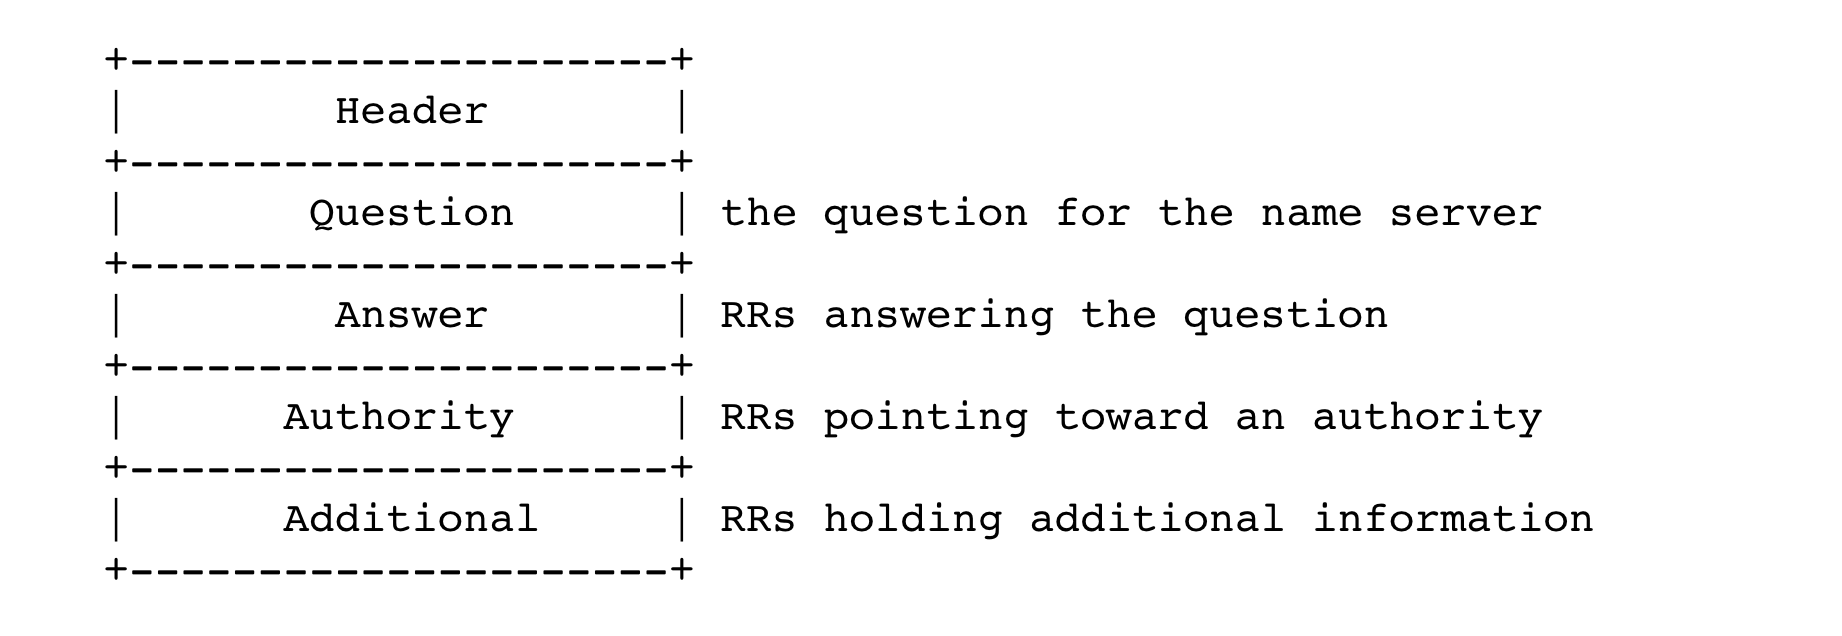
\includegraphics[width=16cm]{dns-message-structure}
\centering
\caption{4.1. Format | RFC 1035}
\end{figure}

\pagebreak

\begin{figure}[h]
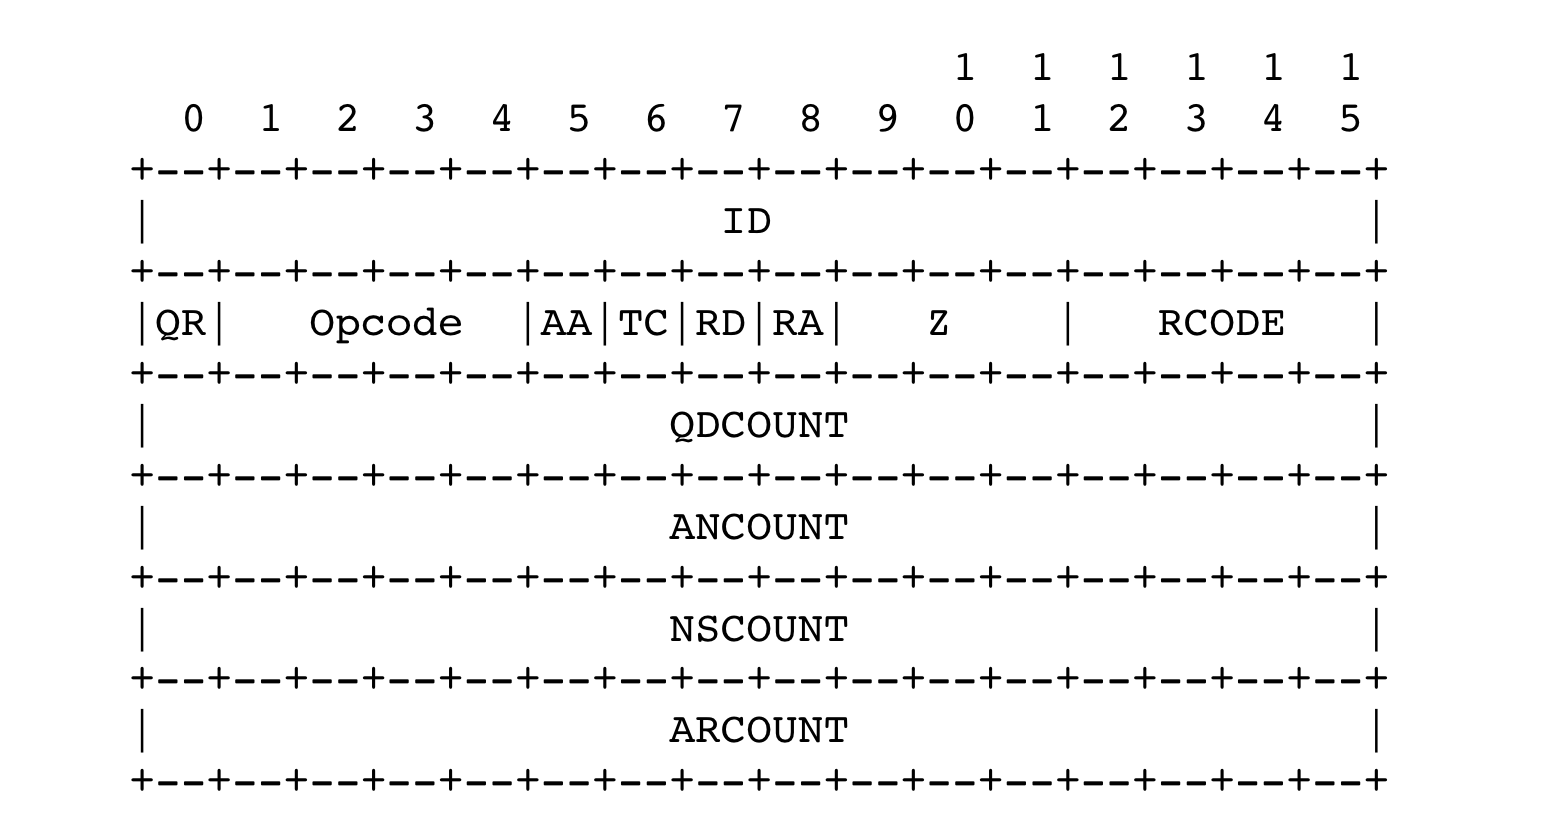
\includegraphics[width=10cm]{dns-header}
\centering
\caption{4.1.1. Header section format | RFC 1035}
\end{figure}

\textbf{DNS Header} has a fixed length, therefore its data structure representation can be easily casted upon the raw data.
Header includes significant meta data about the message, such as the number of questions and answers it carries 
or whether the message is a query or a response or even flags signaling corrupted or invalid messages.
This can be used for more directed parsing and filtering out those messages that this project doesn't care about.

\vspace{1cm}
\begin{figure}[h]
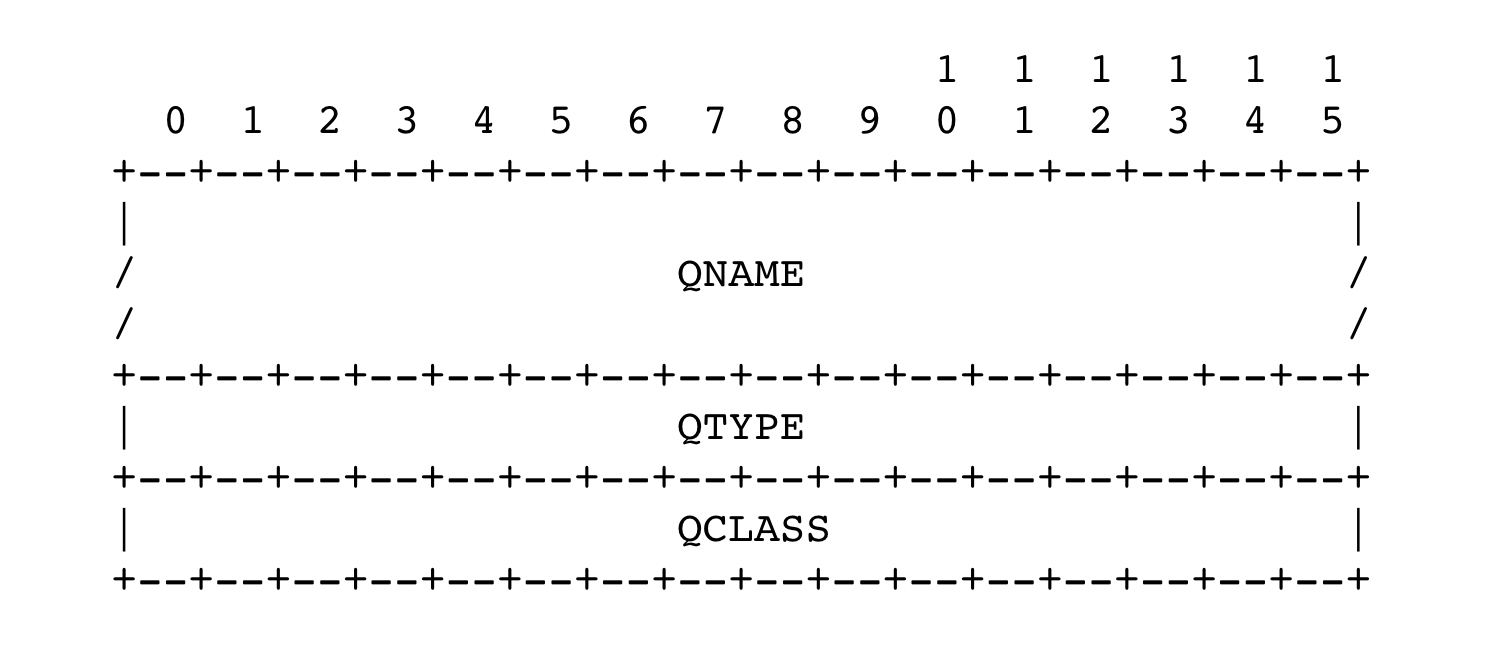
\includegraphics[width=10cm]{dns-question}
\centering
\caption{4.1.2. Question section format | RFC 1035}
\end{figure}

\textbf{Question section} of every DNS packet should contain an initial query record. 

Queries records contain three fields: \textit{QNAME}, \textit{QTYPE} and \textit{QCLASS}.

\vspace{1cm}
\begin{figure}[H]
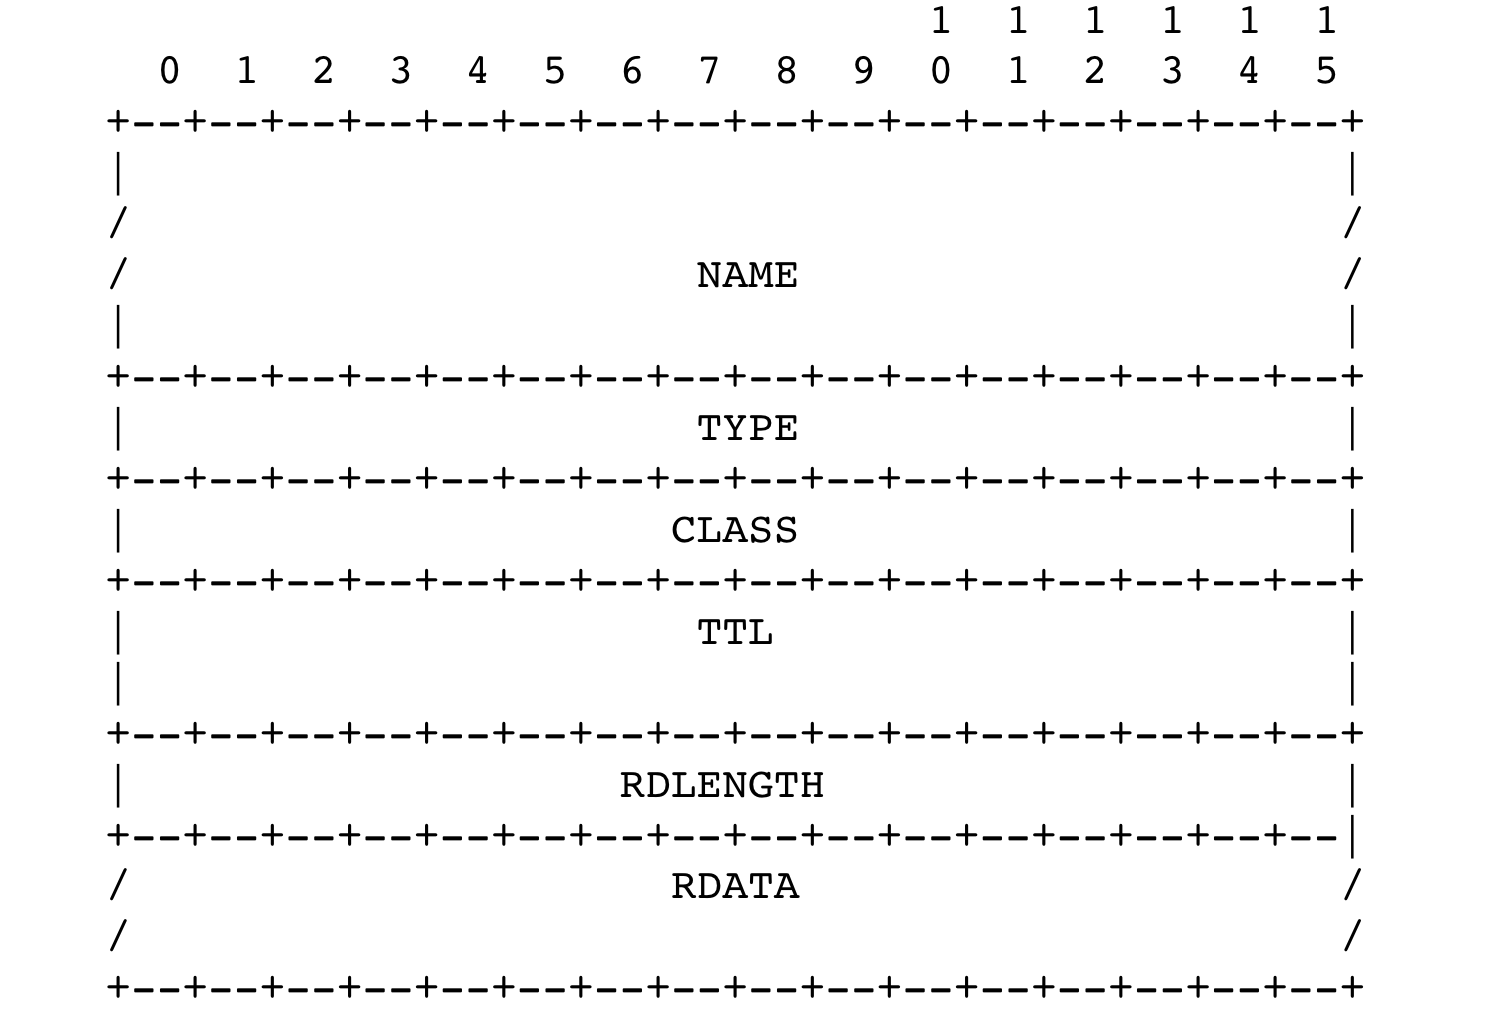
\includegraphics[width=8cm]{dns-rr}
\centering
\caption{4.1.3. Resource record format | RFC 1035}
\end{figure}

\textbf{Answer section} is the most meaningful section of a DNS message, as it contains the valuable response/responses for each query.
Answer sections shares the same format of resource records as the two other sections following it (Authority and Additional), however they are not used in this project.
Answers contain three fields: \textit{NAME}, \textit{TYPE}, \textit{CLASS}, \textit{TTL}, \textit{RDLENGTH} and \textit{RDATA}.

\textbf{RDATA} holds the actual response value during a DNS communication.
It can be represeted in various formats according to the DNS message type.

In this project, these DNS record types will be supported:
\begin{itemize}
\item \textbf{A} - Address record 
\item \textbf{AAAA} - IPv6 address record
\item \textbf{CNAME} - Canonical name record
\item \textbf{NS} - Name server record
\item \textbf{SOA} - Start of authority record
\item \textbf{PTR} - Pointer record
\item \textbf{MX} - Mail exchange record
\item \textbf{TXT} - Text record
\item \textbf{RRSIG} - DNSSEC signature
\item \textbf{NSEC} - Next Secure record
\item \textbf{DS} - Delegation signer
\item \textbf{DNSKEY} - DNS Key record
\end{itemize}

\vspace{0.5cm}

For all of these records, there should be a specific parser implemented. 
The parser will output a string in a readable format and together 
with the question name and type of the message, will be stored in a statistics collection.
If the same DNS resource record will be collected multiple times, 
its count will increase rather than being inserted into the collection redundantly.

\pagebreak

\textbf{Exporting to a Syslog server}

The final task is to export collected statistics one by one to a foreign syslog server, if it was specified.
This simply means, that the application will create a new UDP socket, on which it will send simple messages 
in the official Syslog format specified in RFC 5424.

Example of a syslog message:

\texttt{<134>1 2018-09-20T22:14:15.003Z 192.0.2.1 dns-export - - - goo.gl A 172.217.23.238 5}

This message contains: \texttt{priority, version, datetime, hostname, executable and msg}

\pagebreak

\subsection{Requirements}

Functional requirements from the assignment.
\begin{table}[H]
\centering
\caption{Requirements}
\label{my-label}
\resizebox{\textwidth}{!}{%
\begin{tabular}{@{}|l|l|@{}}
\toprule
\textbf{ID} & \textbf{DESCRIPTION} \\ \midrule
\textit{REQ\_01} & Aplication will process DNS protocol packets. \\ \midrule
\textit{REQ\_01\_01a} & Application will parse relevant link layer protocols (Ethernet, Linux SLL) \\ \midrule
\textit{REQ\_01\_01b} & Application will skip other link layer protocol types. \\ \midrule
\textit{REQ\_01\_02a} & Application will parse relevant network layer protocols (IPv4, IPv6) \\ \midrule
\textit{REQ\_01\_02b} & Application will skip other network layer protocol types. \\ \midrule
\textit{REQ\_01\_03a} & Application will parse relevant transport layer protocols (UDP, TCP) \\ \midrule
\textit{REQ\_01\_03b} & Application will skip other transport layer protocol types. \\ \midrule
\textit{REQ\_01\_04a} & Application will parse just DNS protocol on the application layer. \\ \midrule
\textit{REQ\_01\_04b} & Application will skip other application protocol types. \\ \midrule
\textit{REQ\_01\_05a} & Application will parse A, AAAA, CNAME, MX, NS, SOA, TXT, SPF, DNSKEY, NSEC, RRSIG and DS record types \\ \midrule
\textit{REQ\_01\_05b} & Application will skip other record types. \\ \midrule
\textit{REQ\_02} & Application will collect statistics about selected DNS messages. \\ \midrule
\textit{REQ\_02\_01} & Statistics will take this form: domain-name rr-type rr-answer count \\ \midrule
\textit{REQ\_03} & Application will export statistics to a specified syslog server. \\ \midrule
\textit{REQ\_04} & Application will be run as a executable in CentOS environment from the command line \\ \midrule
\textit{REQ\_05} & Application must accept arguments {[}-r file.pcap{]} {[}-i interface{]} {[}-s syslog-server{]} {[}-t seconds{]} \\ \midrule
\textit{REQ\_05\_01} & Application accepts -h argument for help \\ \midrule
\textit{REQ\_06} & Application will act accordingly to specified arguments \\ \midrule
\textit{REQ\_06\_01} & If interface argument is set, application will listen on a network interface. \\ \midrule
\textit{REQ\_06\_01\_01} & If syslog-server argument is also set, application will export statistics in regular intervals. \\ \midrule
\textit{REQ\_06\_01\_01a} & If seconds argument is also set, interval of statistics exporting is defined by this argument. \\ \midrule
\textit{REQ\_06\_01\_01b} & If seconds argument is not set, interval of statistics exporting is implicitly 60 seconds. \\ \midrule
\textit{REQ\_06\_01\_02} & If syslog-server argument is not set, application will only collect statistics \\ \midrule
\textit{REQ\_06\_02} & If file argument is set, application will read from a static .pcap file. \\ \midrule
\textit{REQ\_06\_02\_01} & Application should accept only .pcap files, or return error when pcap analysis doesn't accept the file. \\ \midrule
\textit{REQ\_06\_02\_02} & If syslog-server argument is also set, application will export statistics at the end of analysis. \\ \midrule
\textit{REQ\_06\_02\_03} & If syslog-server argument is not set, application will print out statistics to the standard output at the end of analysis. \\ \midrule
\textit{REQ\_06\_03} & Combination of interface and file arguments is forbidden. \\ \midrule
\textit{REQ\_06\_03} & Combination of file and seconds arguments is forbidden. \\ \midrule
\textit{REQ\_07} & Application will handle SIGUSR1 signal and print statistics to the standard output. \\ \midrule
\textit{REQ\_08} & Application will handle SIGINT signal and exit. \\ \midrule
\textit{REQ\_09} & Application will create syslog messages from collected statistics. \\ \midrule
\textit{REQ\_09\_01} & Syslog messages will be constructed with syntax according to RFC 5424 \\ \midrule
\textit{REQ\_09\_02} & Required fields are: timestamp, hostname, priority, version, executable name and the actual message data \\ \midrule
\textit{REQ\_09\_03} & Facility must be set to local0. \\ \midrule
\textit{REQ\_09\_04} & Severity must be set to Informational. \\ \midrule
\textit{REQ\_09\_05} & Application will send each statistic in a separate syslog message. \\ \midrule
\end{tabular}%
}
\end{table}

\pagebreak

\subsection{Solution}

Application is able to run in two modes:
\begin{enumerate}
\item Static file analysis
\item Live interface analysis
\end{enumerate}

For the "live" mode, there is a need for a separate thread of processing, as the timer will dispatch messages while the packet analysis still goes on.
To allow both threads to access statistics, stored in a vector structure, there will be a pointer to this structure placed in a global scope.

\vspace{1cm}
\textbf{Approximate structure of the application: }

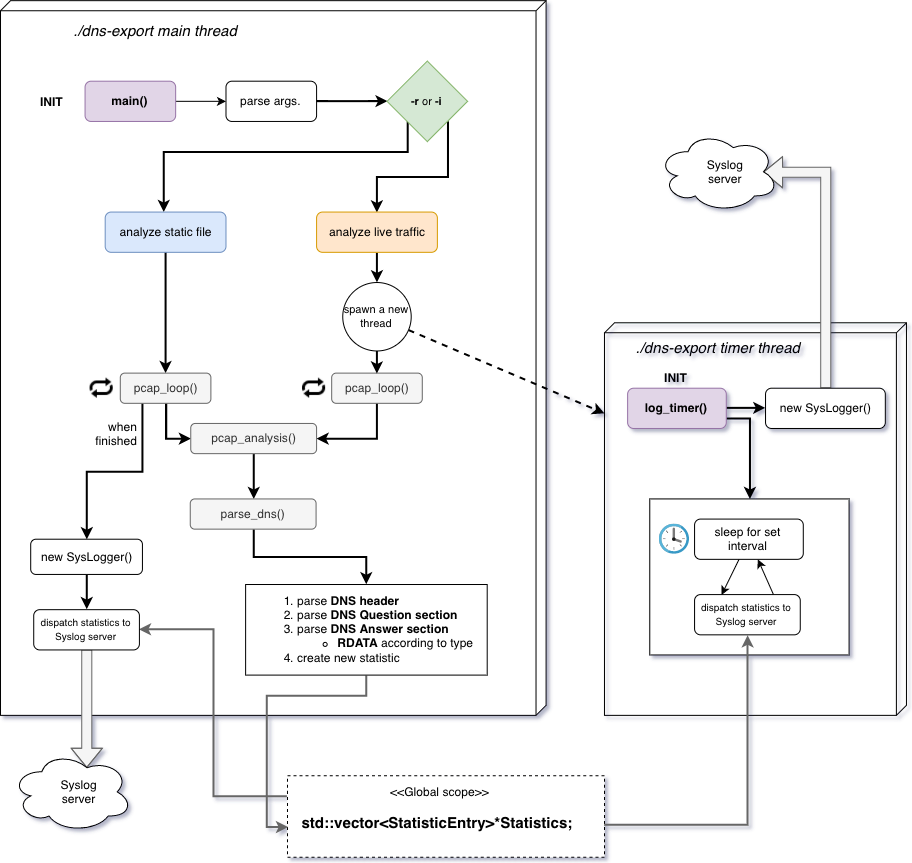
\includegraphics[width=\textwidth]{dns-diagram}

\section{Implementation}

\subsection{Project structure}

\dirtree{%
.1 \faFolderOpen \hspace{1pt} /.
.2 \faFolderOpen \hspace{1pt} src/.
.3 \faFile \hspace{1pt} base64.h.
.3 \faFile \hspace{1pt} config.h.
.3 \faFile \hspace{1pt} dns-header.h.
.3 \faFile \hspace{1pt} misc.h.
.3 \faFile \hspace{1pt} parse-dns.h.
.3 \faFile \hspace{1pt} pcap-analysis.h.
.3 \faFile \hspace{1pt} satistics.h.
.3 \faFile \hspace{1pt} syslogger.h.
.3 \faFileCodeO \hspace{1pt} base64.cc.
.3 \faFileCodeO \hspace{1pt} config.cc.
.3 \faFileCodeO \hspace{1pt} dns-export.cc.
.3 \faFileCodeO \hspace{1pt} parse-dns.cc.
.3 \faFileCodeO \hspace{1pt} pcap-analysis.cc.
.3 \faFileCodeO \hspace{1pt} satistics.cc.
.3 \faFileCodeO \hspace{1pt} syslogger.cc.
.2 \faFileTextO \hspace{1pt} dns-export.1.
.2 \faCogs \hspace{1pt} Makefile.
.2 \faFilePdfO \hspace{1pt} manual.pdf.
}

\subsection{Important sections of the code}

Since the primary objective of this project is to process DNS packets, the following functions are the backbone of the whole processing aspect of this application.

\vspace{1cm}
\textbf{Packet processing loop} \textit{(/src/dns-export.cc)}
\begin{lstlisting}[language=C++] 
    // analyze packets returned by the handle
    if (pcap_loop(pcap_handle, -1, pcap_analysis, reinterpret_cast<u_char*>(&link_type)) != 0)
    {
        std::cerr << "packet reading failed" << std::endl;
        return EXIT_FAILURE;
    }
\end{lstlisting}

\vspace{1cm}
\textbf{Parsing of the DNS frame the application layer} \textit{(/src/parse-dns.h)}
\begin{lstlisting}[language=C++] 
   
    /**
     *  @brief Parse DNS frame of the packet
     * 
     *  @param bytes pointer to the packet
     *  @param packet_offset_size current offset in the packet
     */
    void parse_dns(const u_char* bytes, int32_t packet_offset_size);

\end{lstlisting}

\pagebreak

\vspace{1cm}
\textbf{Parsing of DNS Questions \& Answers sections} \textit{(/src/parse-dns.h)}
\begin{lstlisting}[language=C++] 
    /**
     *  @brief Parse a Question in the Questions section on the DNS frame of the packet
     * 
     *  @param bytes pointer to the packet
     *  @param packet_offset_size current offset in the packet
     */
    size_t parse_dns_question(const u_char* bytes, int32_t packet_offset_size);

    /**
     *  @brief Parse an Answer in the Answers section in the DNS frame of the packet
     * 
     *  @param bytes pointer to the packet
     *  @param packet_offset_size current offset in the packet
     */
    int32_t parse_dns_answer(const u_char* bytes, int32_t packet_offset_size);
\end{lstlisting}

\vspace{1cm}
\textbf{Parsing of RDATA field in DNS Answers section} \textit{(/src/parse-dns.h)}
\begin{lstlisting}[language=C++] 
    /**
     *  @brief Parse the Record Data field in the DNS frame 
     * 
     *  @param bytes pointer to the packet
     *  @param packet_offset_size current offset in the packet
     *  @param type DNS RR type 
     *  
     *  @return parsed RDATA
     */
    std::string parse_dns_answer_rdata( const u_char* bytes, int32_t packet_offset_size, uint16_t rdata_length, uint16_t type);
\end{lstlisting}

\vspace{1cm}
\textbf{Parsing of the domain-name type of fields} \textit{(/src/parse-dns.h)}
\begin{lstlisting}[language=C++]
    /**
     *  @brief Parse the label/ptr name field in the DNS frame
     * 
     *  @param bytes pointer to the packet
     *  @param packet_offset_size current offset in the packet
     *  @param name string to which the parsed content will be stored
     *  @param is_pointer_reference flag describing the context in which the name parsing is run
     *  @param depth of the recursive pointer call
     * 
     *  @return updated packet_offset_size
     */
    int32_t parse_dns_name_field(const u_char* bytes, 
                                int32_t packet_offset_size, 
                                std::string &name, 
                                bool is_pointer_reference,
                                uint8_t depth = 0);
\end{lstlisting}

\vspace{1cm}
\textbf{Parsing of the character-string type of fields} \textit{(/src/parse-dns.h)}
\begin{lstlisting}[language=C++]
    /**
     *  @brief Parse one or more <character-string>s and save them into a string
     * 
     *  @param bytes pointer to the packet
     *  @param packet_offset_size current offset in the packet
     *  @param name string to which the parsed content will be stored
     * 
     *  @return updated packet_offset_size
     */
    size_t parse_dns_string(const u_char* bytes, int32_t packet_offset_size, std::string &name);
\end{lstlisting}

\subsection{Runtime flow structure}

\begin{enumerate}
\item declarations, signals, globals setup
\item argument parsing
\item execution mode split
\begin{enumerate}[label=(\alph*)]
\item interface sniffing
\begin{enumerate}
\item create pcap handle
\item set options for sniffing
\item compile \& apply filter ("port 53")
\item create new thread for regular exporting
\item start analyzing packets
\end{enumerate}
\item offline file reading
\begin{enumerate}
\item open the file
\item start analyzing packets
\end{enumerate}
\end{enumerate}
\item exit
\end{enumerate}

\subsection{Limitations}

\begin{enumerate}
\item Application doesn't support TCP fragmentation of packets.
\item Application doesn't support other link layer types than Ethernet \& Linux SLL
\item 
\end{enumerate}


\section{Usage}

\subsection{Execution details}

After successfuly building the project using \textbf{Makefile}, application can be executed from a command line environment.

To collect statistics from a \textbf{live interface}, use the \textbf{-i} argument and specify the interface name.
To display statistics collected so far during a live capture, send SIGUSR signal to the process of the running application.
To stop collecting statistics and exit from the apllication, send SIGINT signal to the application (for example using CTRL+C inside the terminal).
To change the time for regular statistic dispatching, use the \textbf{-t} argument.

To process an \textbf{offline *.pcap file}, use the \textbf{-r} argument and specify a path to the file.

To specify the syslog server for statistics export, use the \textbf{-s} argument and specify either hostname or ipv4/ipv6 address pointing to the server.

\subsection{Examples}

\vspace{0.5cm}
\textbf{Analyze static file, print statistics to STDOUT}
\begin{lstlisting}[language=Bash] 
./dns-export -r example.pcap
\end{lstlisting}

\vspace{0.5cm}
\textbf{Analyze static file, export to server defined by a hostname}
\begin{lstlisting}[language=Bash] 
./dns-export -r example.pcap -s syslog_sever_domain
\end{lstlisting}

\vspace{0.5cm}
\textbf{Analyze static file, export to server defined by IPv4 address}
\begin{lstlisting}[language=Bash] 
./dns-export -r example.pcap -s 127.0.0.1
\end{lstlisting}

\vspace{0.5cm}
\textbf{Analyze static file, export to server defined by IPv6 address}
\begin{lstlisting}[language=Bash] 
./dns-export -r example.pcap -s ::1
\end{lstlisting}

\vspace{0.5cm}
\textbf{Analyze live traffic from an interface}
\begin{lstlisting}[language=Bash] 
./dns-export -i en0
\end{lstlisting}

\vspace{0.5cm}
\textbf{Analyze live traffic from an interface, set timer to 5 seconds}
\begin{lstlisting}[language=Bash] 
./dns-export -i en0 -t 5
\end{lstlisting}

\vspace{0.5cm}
\textbf{Analyze live traffic from an interface, export to a syslog server defined by a hostname}
\begin{lstlisting}[language=Bash] 
./dns-export -i en0 -s syslog_server_domain
\end{lstlisting}

\vspace{0.5cm}
\textbf{Analyze live traffic from an interface, export to a syslog server defined by a hostname and set the timer to 5 seconds}
\begin{lstlisting}[language=Bash] 
./dns-export -i en0 -s syslog_server_domain -t 5
\end{lstlisting}



\section{Acknowledgments / Sources}

The work done on this project was supported by the following sources, guides and code samples.

\subsection{Theoretical understanding}


\subsubsection{Online articles and guides}

\url{https://0x00sec.org/t/how-do-those-hackers-tools-work-sniffers-part-i/686}

\url{https://0x00sec.org/t/how-do-those-hackers-tools-work-sniffers-part-ii/777/4}

\subsubsection{Official documentations and RFCs}

\url{https://www.tcpdump.org/linktypes.html}

\url{https://www.tcpdump.org/manpages/pcap.3pcap.html}

\href{https://www.ietf.org/rfc/rfc1035.txt}{RFC 1035 - DOMAIN NAMES - IMPLEMENTATION AND SPECIFICATION}

\href{https://tools.ietf.org/html/rfc3596}{RFC 3596 - DNS Extensions to Support IP Version 6}

\href{https://www.ietf.org/rfc/rfc4034.txt}{RFC 4034 - Resource Records for the DNS Security Extensions}

\href{https://tools.ietf.org/html/rfc5424}{RFC 5424 - The Syslog Protocol}

\pagebreak

\subsection{Used libraries}

This project makes use of these STD C++ libraries:

\begin{lstlisting}[language=C++] 
#include <memory>
#include <iostream>
#include <iomanip>
#include <string>
#include <unistd.h>
#include <vector>
#include <thread>
#include <chrono>
#include <sstream>
#include <signal.h>
#include <sys/socket.h>
#include <pcap.h>
#include <netinet/in.h>
#include <netinet/ip.h>
#include <netinet/tcp.h>
#include <netinet/udp.h>
#include <netinet/if_ether.h>
#include <arpa/inet.h>
#include <netinet/ether.h> 
#include <time.h>
#include <pcap/pcap.h>
#include <syslog.h>
#include <sys/types.h>
#include <sys/socket.h>
#include <unistd.h>
#include <time.h>
#include <netdb.h>
\end{lstlisting}


\subsection{External source code}

For the \textbf{Base64 encoding}, which is used when parsing DNSSEC records, I acknowledge the use of a source code by René Nyffeneggerhis under the specified license conditions.

\url{https://renenyffenegger.ch/notes/development/Base64/Encoding-and-decoding-base-64-with-cpp}

\vspace{1cm}
For the \textbf{DNS header structure}, which is used when parsing the DNS header section of every packet, I acknowledge the use of a source code from this location:

\url{https://0x00sec.org/t/dns-header-for-c/618}

Use of this resource is permitted by it's author without any limitations.


\end{document}